No dataset specifically containing a known list of codewords in the way I defined exists. This frustrates research efforts since a dataset is needed to establish baselines and run experiments. Hence, I created a synthetic dataset for this problem.

\subsection{Approach Overview}

\subsubsection{Easy Codeword Corpus}

The general idea is to generate a synthetic codeword corpus $C_c$ from a reference corpus $C_r$. By creating a few codewords in a corpus known not to have many codewords, this method allows me to test codeword detection against the synthetic codewords. The steps are:

\begin{itemize}
\item Get a reference corpus containing little to no codewords (e.g. the WSJ corpus)
\item Select $n$ words in the corpus.
\item For each of these $n$ words (i.e. $w_{i, r}$ for all $i \in 1 ... n$), generate a set of words $w_{j, r}$ where $w_{i, r} \neq w_{j, r}$ for $j \in 1 .. n$. In other words, map each word select to another word in the set of $n$ words.
\item Generate a codeword corpus by replacing all $w_{i, r}$ with $w_{j, r}$.
\end{itemize}

For example, if I select the words ``hello'', ``cheeseburger'', and ``fruit'' in the reference corpus, then ``hello'' could be replaced by ``cheeseburger'', ``cheeseburger'' replaced by ``fruit'', and ``fruit'' replaced by ``hello''. This means that in the synthetic codeword corpus, I would see the sentence ``cheeseburger, have a good day'' instead of ``hello, have a good day''. This captures the first semantic of a codeword: a word being used in a context different than its usual context. In the synthetic corpus, I have created an extreme example -- compared to the reference corpus, all contexts of ``hello'' has been modified to that of ``cheeseburger''s.

\subsubsection{Hard Codeword Corpus}

Alternatively, a ``harder'' codeword corpus can be generated. This captures both semantics of codewords -- both different contexts and specific subgroups of users.

\begin{itemize}
\item Get a reference corpus containing little to no codewords (e.g. the WSJ corpus)
\item Select $n$ words in the corpus.
\item For each of these $n$ words (i.e. $w_{i, r}$ for all $i \in 1 ... n$), generate a set of words $w_{j, r}$ where $w_{i, r} \neq w_{j, r}$ for $j \in 1 .. n$. In other words, map each word select to another word in the set of $n$ words.
\item Generate a codeword corpus by replacing all $w_{i, r}$ with $w_{j, r}$ \textbf{within a specific subset (community) of documents}.
\end{itemize}

For this harder approach, one could imagine an already partitioned corpus (such as Reddit, where each forum (subreddit) is grouped into a single community). Then, replacements are only done to words in a community, but not to words outside those community. Hence, ``hello'' will be replaced by ``cheeseburger'' only within, say, the \texttt{/r/gaming} community, but not in everything else.

There are two problems to tackle:

\begin{enumerate}
\item What reference corpus should I use to generate the synthetic corpus from
\item How do I select salient, important words to be used as codewords (not words such as ``the'' and ``he''
\end{enumerate}

These will be addressed in the next section.

\subsection{Reference Corpus choice}

I choose the WSJ Corpus from the PennTreebank to be the reference corpus due to the similarity in the content of the text and the data of potential clients. A helper function is made in \lstinline{lib.corpus_parser} to use \lstinline{nltk} to parse the WSJ corpus. Tip to future replications: use a symlink to link \lstinline{LDC99T42-Treebank-3/package/treebank 3/parsed/mrg/wsj} and \lstinline{LDC99T42-Treebank-3/package/treebank 3/parsed/mrg/brown} to \lstinline{~/nltk data/corpora/ptb/wsj} and \lstinline{~/nltk data/corpora/ptb/brown} so that \lstinline{nltk} can parse the WSJ corpus directly.

For the harder codeword corpus, I used a Reddit dataset scraped from Reddit using a scraper I wrote (\url{github.com/linanqiu/omega-red}). Details of this project is left in the appendix. The advantage of this corpus is that I am able to obtain pre-labeled communities. Reddit forums exist in the form of subreddits and metareddits. Subreddits are individual forums related to a topic, such as football or baseball. Metareddits are groupings of subreddits around a theme, such as news, politics, sports etc. My scraper obtained 5000 threads from each of the following subreddits in each of the following metareddits.

\begin{figure}[h]
\begin{itemize}
\item[news]: politics, worldnews, news, conspiracy, libertarian, truereddit, conservative, offbeat
\item[lifestyle]: food, guns, motorcycles, sex, progresspics, lifehacks, frugal, drunk
\item[learning]: todayilearned, science, askscience, space, askhistorians, youshouldknown, explainlikeimfive
\item[humor]: funny, adviceanimals, imgoingtohellforthis, facepalm, jokes, circlejerk
\item[entertainment]: music, movies, harrypotter, starwars, anime, comicbooks
\item[television]: gameofthrones, doctorwho, mylittlepony, community, breakingbad, startrek, himym, thewalkingdead
\item[gaming]: gaming, leagueoflegends, pokemon, minecraft, starcraft, dota2, skyrim, tf2
\end{itemize}
\caption{Listing of metareddits and subreddits in the reddit corpus. 5000 threads and comments were scraped from each subreddit.}
\label{fig-reddit-corpus}
\end{figure}

As shown in Figure \ref{fig-reddit-corpus}, I obtained a total of 800MB of Reddit data.

\subsection{Selecting Salient Words}

I also needed a way to select $n$ codewords (in this case I used $n = 100$ in most corpus based on intuition about the size of the corpus and usage patterns)

\subsubsection{TF-IDF}

A naive way to do this would be TF-IDF. I used this initially, where

\begin{itemize}
\item $T_{i, r}$ is the number of times word $w_{i, r}$ appeared in the corpus $C_r$
\item $D_{i, r}$ is the number of documents (in the case of WSJ, separate articles) that word $w_{i, r}$ appeared in
\item $N_D$ is the number of documents in the entire corpus
\end{itemize}

Then, each word is assigned a rank $R_{i, r}$ where

\[R_{i, r} = TFIDF_{i, r} = \log{\left(T_{i, r} + 1\right)} * \log{\left(1 + \frac{N_D}{D_{i, r}}\right)}\]

The left term is the term frequency smoothed so that 0s won't occur, and the right term is the inverse document frequency.

We select the top $n$ words with the highest $R_{i, r}$. The intuition behind this method was to downweight terms that appeared in every document (such as ``the'', ``a'', ``he''), and upweight rarer terms.

However, this method was disappointing since it upweighted rare terms too much. In particular, note that the inverse document frequency portion of TFIDF is a decreasing function. That means words appearing only 1 time is upweighted the most. Hence, a lot of names and esoteric words that only occur once were selected. The top words consisted of ``yeargin'', ``steinhardt'', ``corry'', ``psyllium''. We needed an alternative method that downweighted very frequent words, upweighted rarer words, but also downweighted extremely rare words.

\subsubsection{Gamma Weighted TF-IDF}

Instead, I discovered that a good way to do this was to use a Gamma distribution instead of the inverse document frequency measure. That means 

\[R_{i,r} = \log{\left(T_{i, r} + 1\right)} * g\left(D_{i, r}\right)\]

where $g(y)$ is the Gamma distribution function fitted on a given $\alpha$ and $\beta$. Specifically, I can set $\alpha$ and $\beta$ such that the mode of the distribution is a certain proportion of documents (i.e. this is the proportion of documents that ``important words'' should belong in) and the mean to be 2 times of that. Choosing $mode = 0.075*N_D = (\alpha - 1) * \beta$ and hence $mean = 0.15 * N_D = \alpha * \beta$ we make the assumption that important words should be present in around 7.5\% to 15\% of articles. The gamma distribution hence looks like Figure \ref{fig-gamma-dist}.

\begin{figure}[h]
\centering
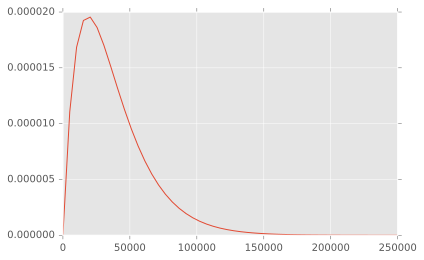
\includegraphics[width=.5\textwidth]{figures/gamma-dist.pdf}
\caption{Gamma distribution $g(x)$ used to upweight important words.}
\label{fig-gamma-dist}
\end{figure}

This function upweights words that appear not so frequently, but downweights words that appear very rarely (along with words that appear frequently). The results turned out to be very reasonable for the WSJ corpus. Top words include ``bonds'', ``index'', ``japanese'', ``oil'', ``traders''.

This result should not be surprising given that TF-IDF is a measure meant for weighting words in a single document among many documents, not an aggregate measure across documents.
This allows us to select $n$ words by taking the top $n = 100$ words using $R_{i,r}$

\subsection{Generating a Substitute Corpus}

Now that I have selected the most salient $n$ words in a corpus, I want to create a matching between $w_{i, r}$ and $w_{j, r}$ as mentioned earlier. This matching should be such that $w_{i, r} \neq w_{j, r}$ for all $i$ and $j$ in $1 ... n$. This is rather trivial, and we simply shuffle the set of $n$ words to get $j$.

Then, we can generate a codeword corpus by going through the reference corpus and replacing every occurrence of word $w_{i, r}$ with $w_{j, r}$.

We generated the following easy and hard synthetic codeword corpora:

\begin{itemize}
\item (Easy) WSJ synthetic corpus generated by replacing 100 words in the entire WSJ corpus
\item (Easy) Reddit synthetic corpus generated by replacing 100 words in the entire reddit corpus
\item (Hard) 7 Reddit community synthetic corpus generated by replacing 100 words in only 1 metareddit (community) of the reddit corpus while leaving the rest of the corpus in tact
\end{itemize}